The project we worked on this semester was the GIRAF project. The following section describes what the project is, as well as the state at handover.

People with an \gls{asd} can have difficulties with communication. GIRAF is a tablet environment developed to ease communication between people with an \gls{asd} and the people who take care of them. In this report we refer to them as \glspl{citizen} and \glspl{guardian}.

Software students develop GIRAF as their bachelor project. The students work in small teams and coordinate the work between teams. The students collaborate with the following institutions \cite{GirafWebsite}, that act as customers in the development process.

\begin{itemize}
    \item Børnehaven Birken (Kindergarten) \cite{bhBirken}
    \item Egebakken (School) \cite{egebakken}
    \item Enterne (Home for disabled) \cite{enterne}
    \item The speech institute at Aalborg municipality
    \item Center for Autism and ADHD \cite{center_for_autism}
\end{itemize}

The project started in 2011 and each year the students continue where the previous years students left off.

This semester started with the decision to, like previous years, run the project with the \gls{Scrum_principles}. One group was appointed \gls{PO} team and another was appointed \gls{SMT}. The \gls{PO} team is responsible for customer communication and the product backlog. The \gls{SMT} decides how the process is defined, and make guidelines for the \glspl{devTeam}.

\section{Current state of GIRAF}

We got the work from previous teams in the beginning for the semester. This section describes the product at this stage, and explains the elements that is important to follow the rest of the report.

Earlier, the GIRAF project contained several applications. These shared the same backend. The \glspl{devTeam} in 2017 changed the system backend\cite{SW608F18} and left all applications unusable, because the \gls{api} they used was no longer accessible and the new \gls{api} was not backwards compatible. They rebuild a application called the Weekplanner, but did not have time to get the other applications to work. 

Since then the Weekplanner is the only application that have been worked on, and also the one the costumers showed by far the most interest. We decided to limit our development to the weekplanner. 


The backend is a .NET Core 2 project that uses traditional MVC and supports all the capabilities of the current Weekplanner app. It exposes a REST-inspired API to the front end.
\begin{figure}[H]
        \begin{center}
            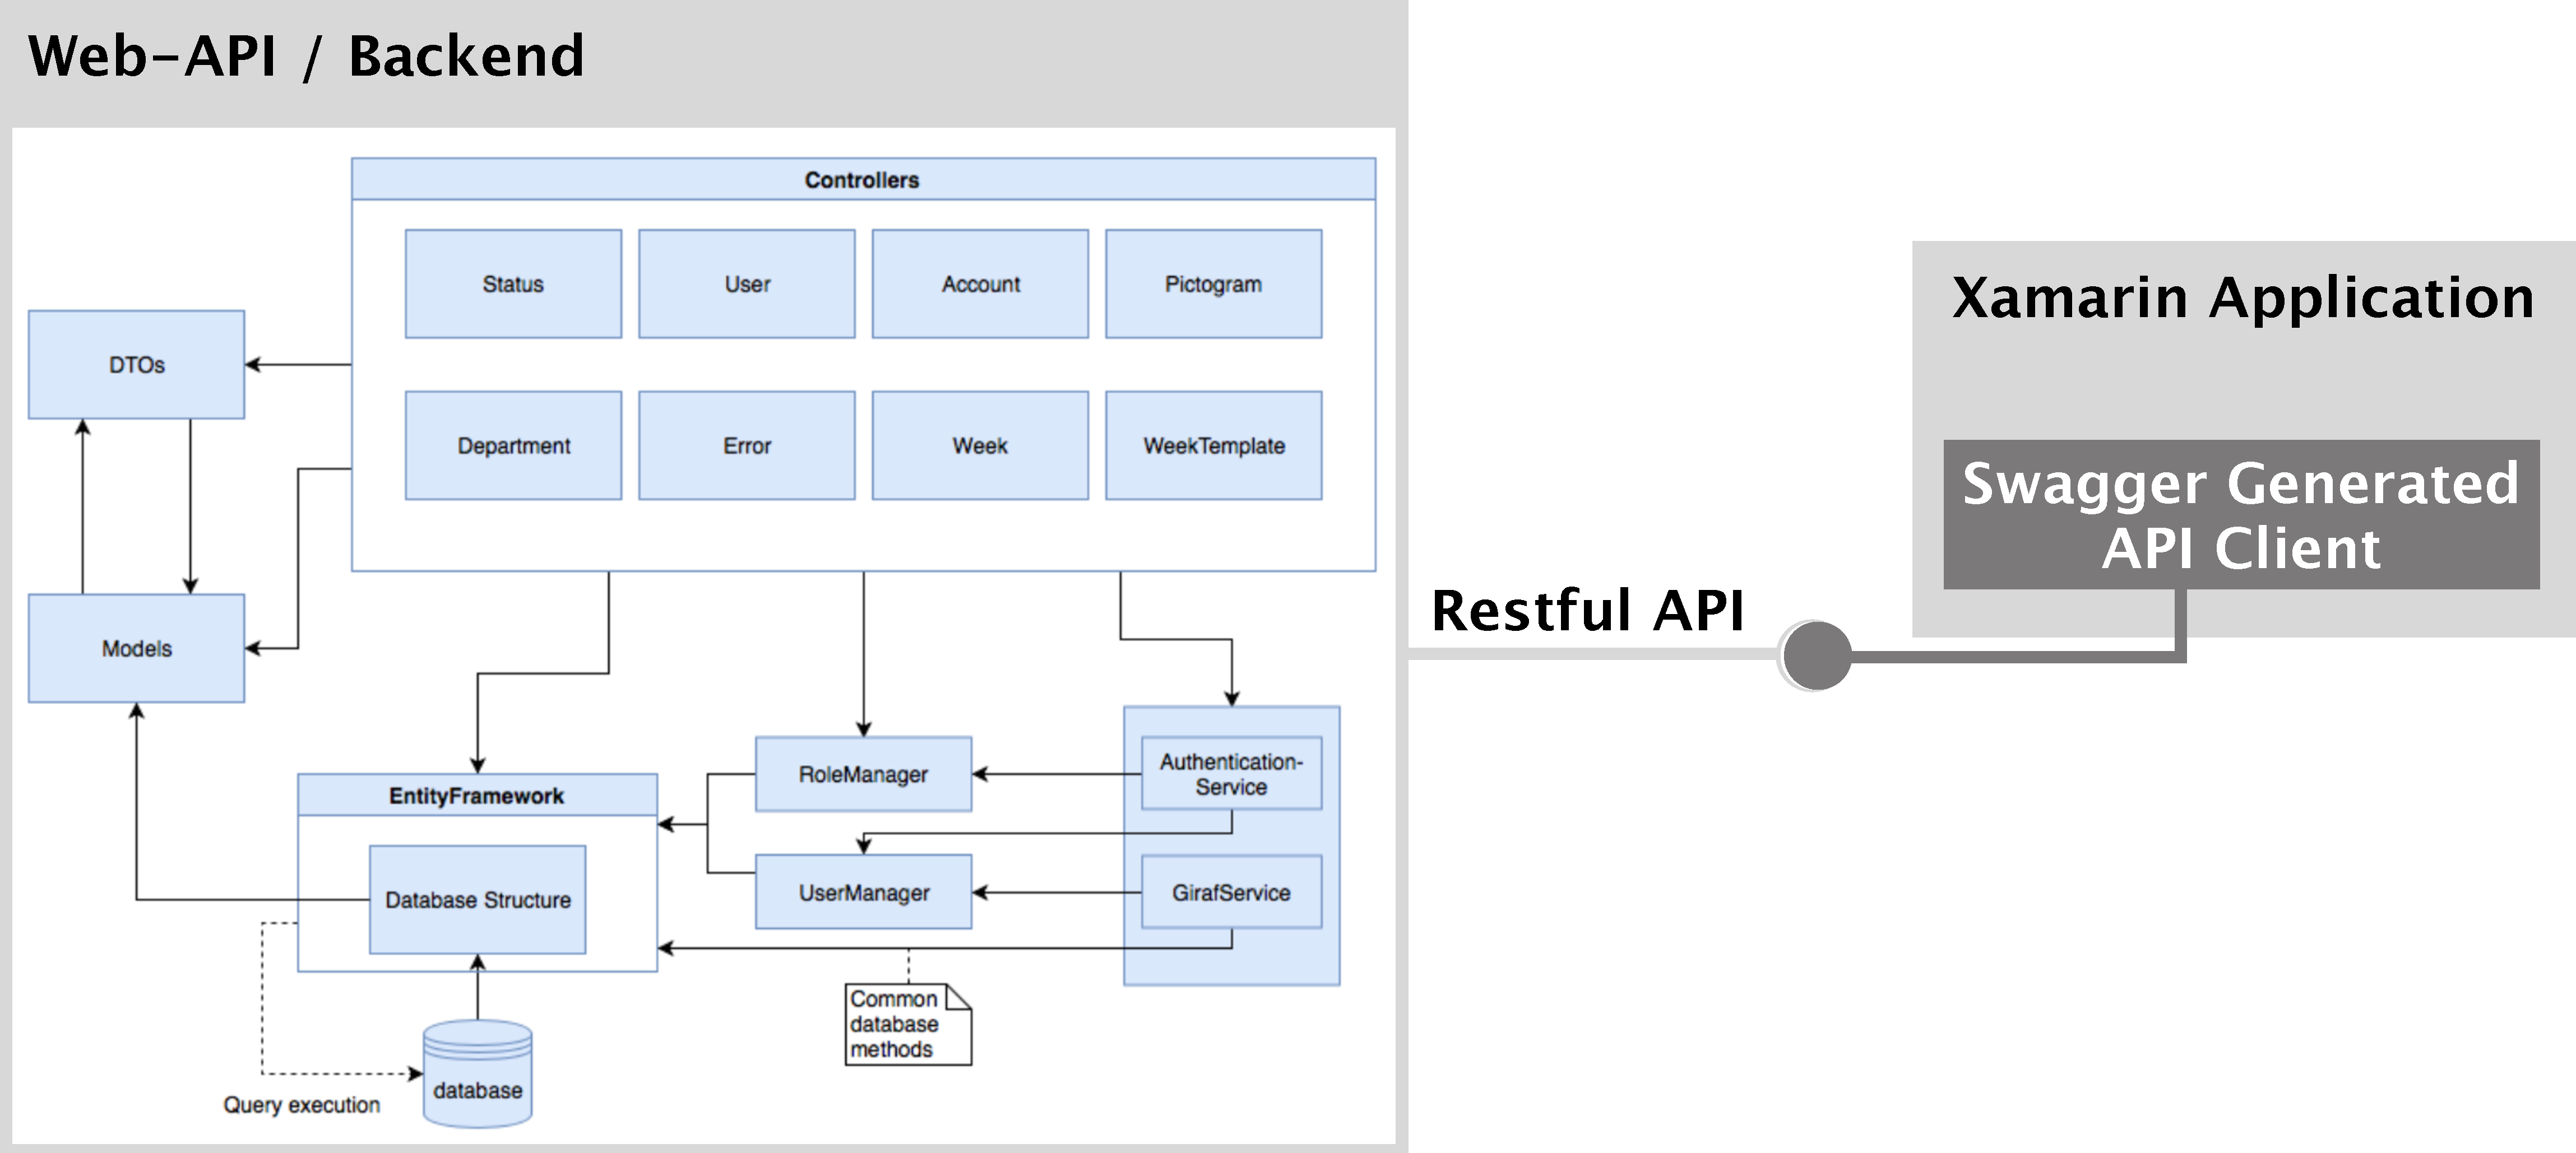
\includegraphics[width=0.95\textwidth]{figures/RestAPIFigure.pdf}
        \end{center}
        \caption{Illustration of the .NET Core 2 project and how it exposes a RESTful API}
        \label{fig:RestAPIFigure}
\end{figure}

